\chapter{\ifproject%
\ifenglish Project Structure and Methodology\else โครงสร้างและขั้นตอนการทำงาน\fi
\else%
\ifenglish Project Structure\else โครงสร้างของโครงงาน\fi
\fi
}


ในบทนี้จะกล่าวถึงหลักการ และการออกแบบระบบ

\makeatletter

% \renewcommand\section{\@startsection {section}{1}{\z@}%
%                                    {13.5ex \@plus -1ex \@minus -.2ex}%
%                                    {2.3ex \@plus.2ex}%
%                                    {\normalfont\large\bfseries}}

\makeatother
%\vspace{2ex}
% \titleformat{\section}{\normalfont\bfseries}{\thesection}{1em}{}
% \titlespacing*{\section}{0pt}{10ex}{0pt}

\section{หลักการทำงานของระบบ}

\begin{figure}[h!]
\begin{center}
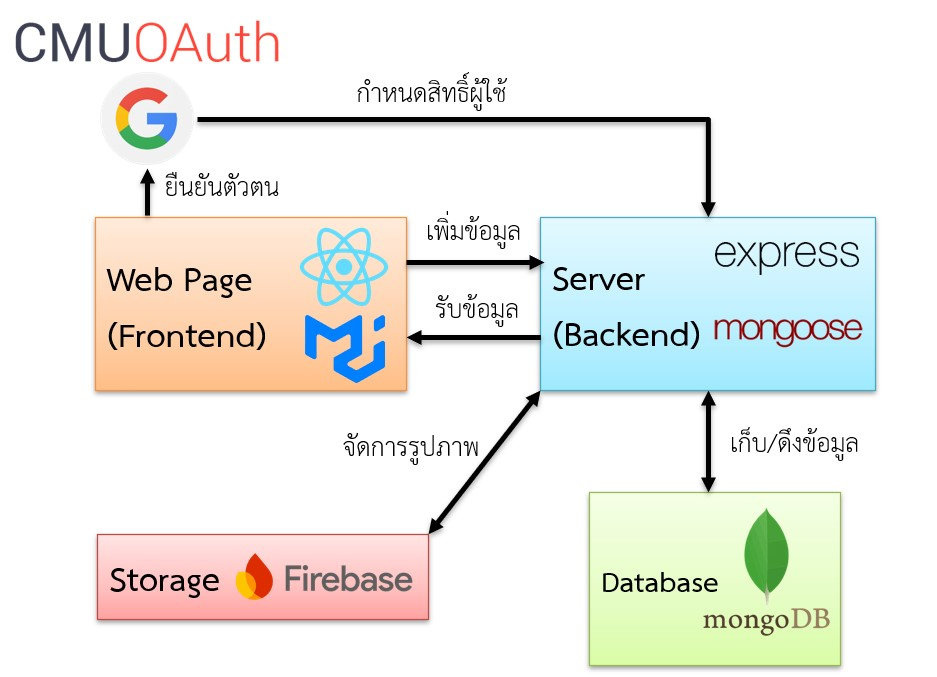
\includegraphics[scale=0.6]{public/sys-overview.jpg}
\end{center}
\caption[Poem]{System Overview}
\label{fig:sys-overview}
\end{figure}

\subsection{ภาพรวมของระบบ (System Overview)}
ภาพรวมการทำงานของระบบ จะมีส่วนประกอบหลักๆ ดังนี้

\bullet{ Frontend}
ประกอบไปด้วย React Framework, โค้ด HTML, Javascript และ Material UI ใช้สำหรับแสดงผลหน้าเว็บให้แก่ผู้ใช้

\bullet{ Backend}
ประกอบไปด้วย ExpressJS, NodeJS, Mongoose และ Authorization ใช้สำหรับการทำ business logic ของระบบ

\bullet{ Database}
ประกอบไปด้วย MongoDB ใช้สำหรับเก็บข้อมูลของระบบ

\bullet{ Object Storage}
เลือกใช้บริการของ Google Firebase ในการเก็บรูปภาพกิจกรรมต่างๆ

\bullet{ Authentication}
เลือกใช้บริการ OAuth ของ Google และ CMU Account ในการเข้าสู่ระบบ
\clearpage

\subsection{โครงสร้างฐานข้อมูล (Database Schema)}
Database ของระบบนี้ ประกอบไปด้วย 3 Collections ดังนี้

\begin{enumerate}
\item Event Collection: 
\begin{itemize}
  \item Primary Field คือ id
  \item String Fields ได้แก่ ชื่อกิจกรรม, คำอธิบายกิจกรรม, สถานที่, อีเมล, เบอร์โทรศัพท์ และ ช่องทางติดต่ออื่นๆ
  \item Array Fields ได้แก่ ประเภทกิจกรรม, คณะที่สามารถเข้าร่วมได้, path ของรูปภาพกิจกรรม และ สถานะการประกาศ
  \item Date Fields ได้แก่ วัน/เวลาเริ่มต้นกิจกรรม, วัน/เวลาสิ้นสุดกิจกรรม, วัน/เวลาประกาศกิจกรรม และ วัน/เวลาแก้ไขรายละเอียดกิจกรรม
  \item Boolean Field คือ การประกาศจากคณะ/หน่วยงาน
  \item createdBy อ้างอิงถึง Primary Field ของ User Collection (\_id)
\end{itemize}
\item User Collection:
\begin{itemize}
  \item Primary Field คือ \_id
  \item String Fields ได้แก่ ชื่อผู้ใช้, อีเมล, path ของรูป profile
  \item Array Field คือ แท็กที่ผู้ใช้สนใจ
  \item Date Fields ได้แก่ วัน/เวลาสร้างบัญชี และ วัน/เวลาแก้ไขบัญชี
  \item เนื่องจากเราใช้บริการ OAuth จึงไม่ต้องเก็บข้อมูลรหัสผ่าน
\end{itemize}
\item Review Collection: 
\begin{itemize}
  \item Primary Field คือ id
  \item user\_id อ้างอิงถึง Primary Field ของ User Collection (\_id)
  \item event\_id อ้างอิงถึง Primary Field ของ Event Collection (id)
  \item Number Field จะเก็บคะแนนในเกณฑ์ต่างๆ ได้แก่ เนื้อหา, วัน/เวลา, สถานที่ และ ทีมงาน
  \item status ใช้ระบุว่าผู้ใช้ได้กดสนใจหรือไม่
\end{itemize}
\end{enumerate}

\begin{figure}[H]
\begin{center}
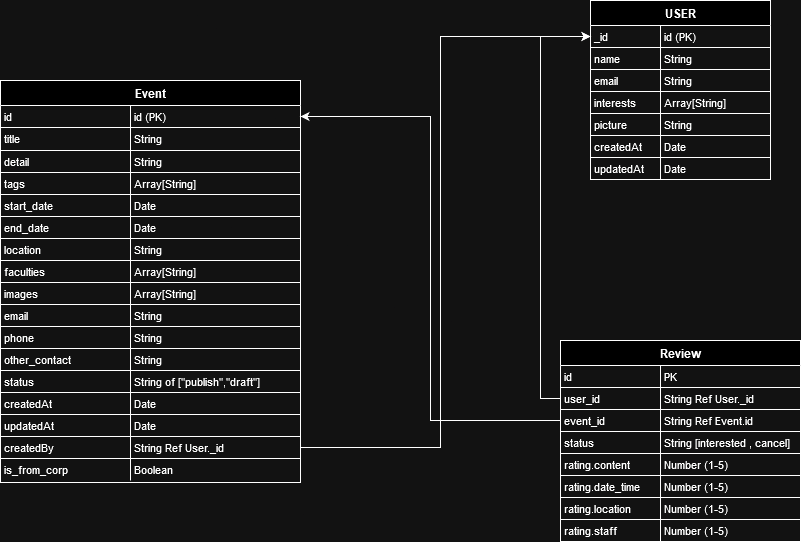
\includegraphics[scale=0.4]{public/db-diagram.png}
\end{center}
\caption[Poem]{Schema Diagram}
\label{fig:db-schema}
\end{figure}
\section{ส่วนเชื่อมต่อระหว่างผู้ใช้งานกับระบบ (User Interface)}
\subsubsection{หน้าแรก (Landing Page)}

\begin{figure}[H]
\begin{center}
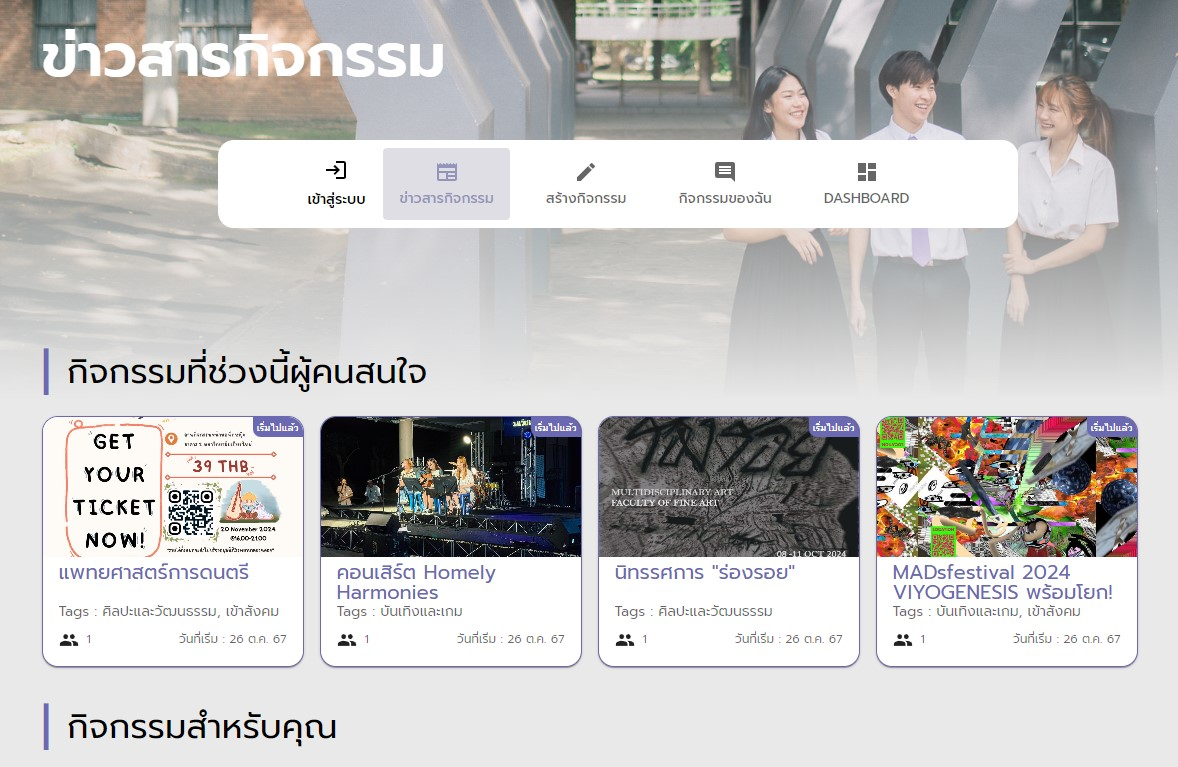
\includegraphics[scale=0.5]{public/landing.jpg}
\end{center}
\caption[Poem]{Landing Page}
\label{fig:landing-page}
\end{figure}
\clearpage
\subsubsection{หน้าเข้าสู่ระบบ (Login Page)}
เมื่อกดปุ่มเข้าสู่ระบบในหน้าแรก จะเปลี่ยนมาเป็นหน้านี้
\begin{figure}[H]
\begin{center}
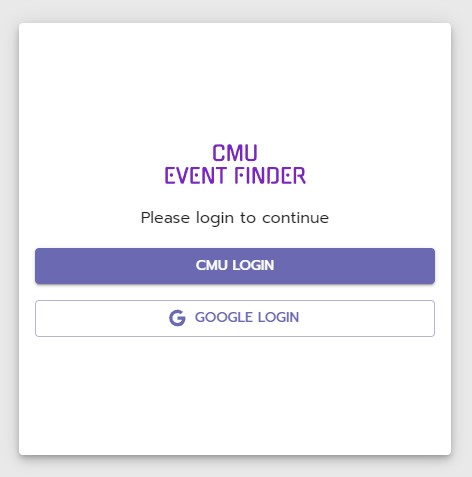
\includegraphics[scale=0.6]{public/login-page.jpg}
\end{center}
\caption[Poem]{Login Page}
\label{fig:login-page}
\end{figure}

\subsubsection{หน้าสร้างกิจกรรม (Create Event Page)}
\begin{figure}[H]
\begin{center}
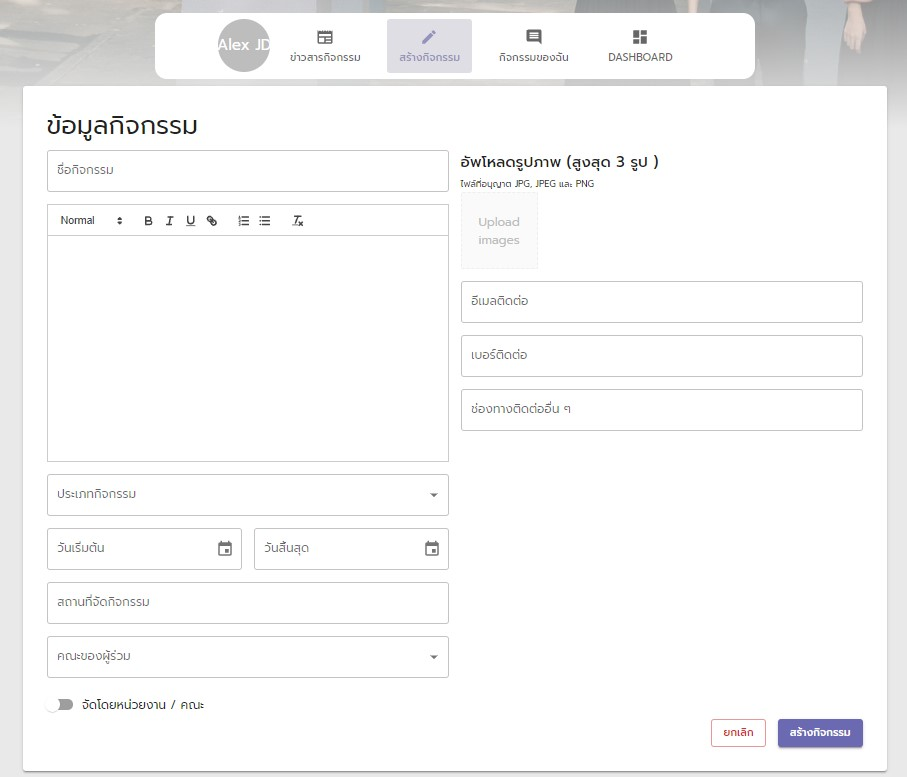
\includegraphics[scale=0.6]{public/create-act.jpg}
\end{center}
\caption[Poem]{Create Event Page}
\label{fig:create-page}
\end{figure}
\clearpage
\subsubsection{หน้ากิจกรรมของฉัน (Create Event Page)}
ประกอบด้วยกิจกรรมที่สร้าง และกิจกรรมที่กดสนใจเข้าร่วม
\begin{figure}[H]
\begin{center}
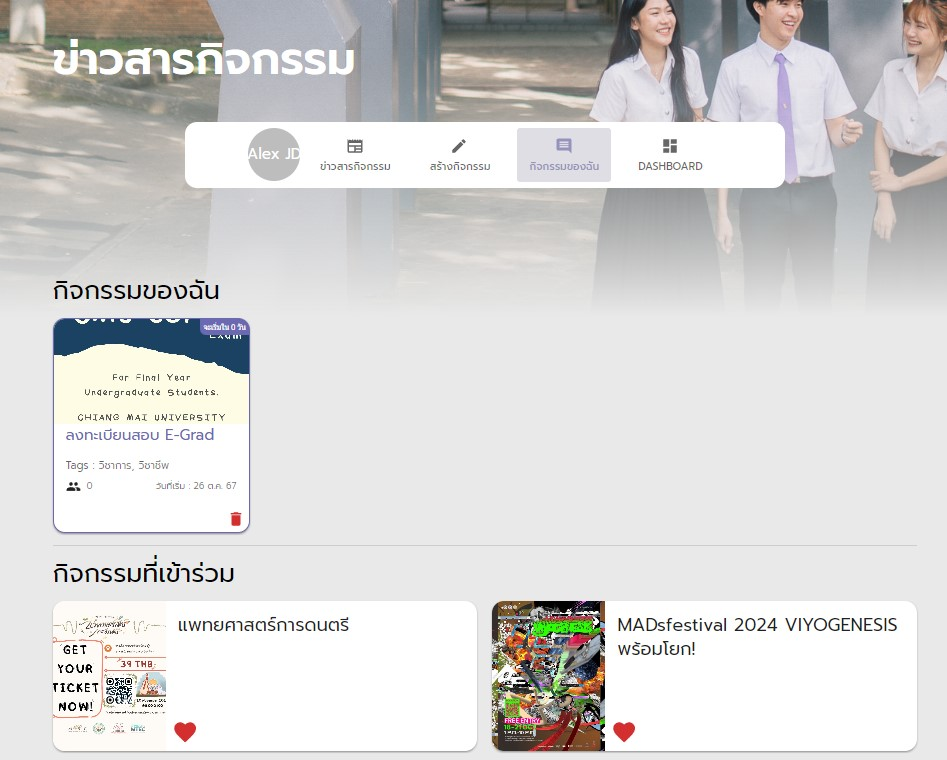
\includegraphics[scale=0.5]{public/my-act.jpg}
\end{center}
\caption[Poem]{My Event Page}
\label{fig:my-event-page}
\end{figure}
\subsubsection{หน้าแดชบอร์ด (Dashboard Page)}
สามารถดูสถิติโดยรวมของเว็บได้
\begin{figure}[H]
\begin{center}
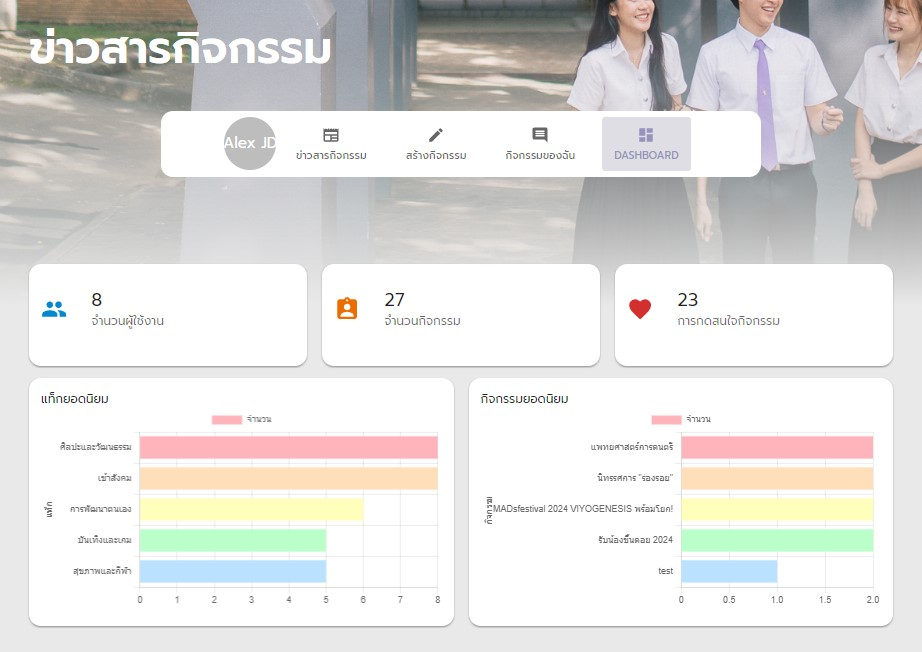
\includegraphics[scale=0.5]{public/dash-page.jpg}
\end{center}
\caption[Poem]{Dashboard Page}
\label{fig:dashboard-page}
\end{figure}
\clearpage
\subsubsection{รายละเอียดกิจกรรม (Event Detail)}
จะแสดงรายละเอียดทั้งหมดของกิจกรรม
\begin{figure}[H]
\begin{center}
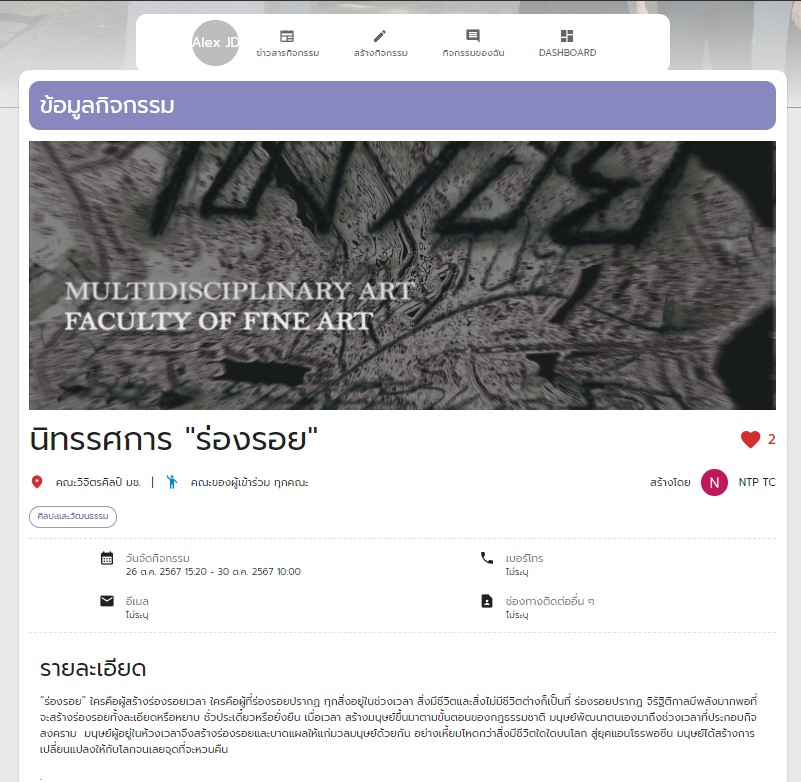
\includegraphics[scale=0.6]{public/act-detail.jpg}
\end{center}
\caption[Poem]{Event Detail}
\label{fig:event-detail}
\end{figure}
\subsubsection{รายละเอียดกิจกรรมโดยย่อ (Event Box)}
จะแสดงรายละเอียดโดยย่อของกิจกรรม
\begin{figure}[H]
\begin{center}
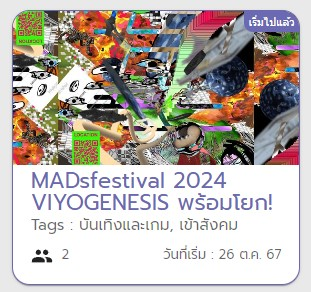
\includegraphics[scale=0.8]{public/act-mini.jpg}
\end{center}
\caption[Poem]{Event Box}
\label{fig:event-box}
\end{figure}
\clearpage
\subsubsection{หน้าต่างรีวิวกิจกรรม (Review Window)}
เมื่อกดปุ่ม "กรุณาให้คะแนน" หน้าต่างรีวิวกิจกรรมจะแสดงขึ้นมา
\begin{figure}[H]
\begin{center}
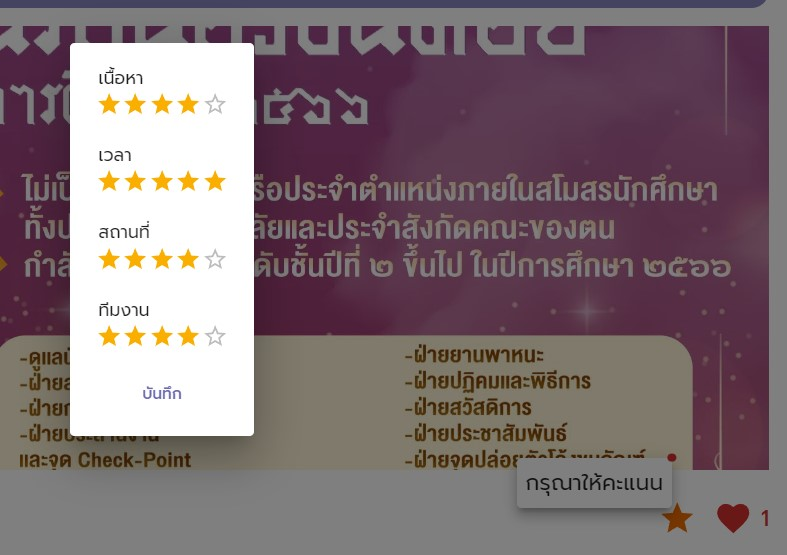
\includegraphics[scale=0.8]{public/act-review.jpg}
\end{center}
\caption[Poem]{Review Window}
\label{fig:review-window}
\end{figure}
\subsubsection{ส่วนแสดงคะแนนกิจกรรม (Score Section)}
ในหน้ารายละเอียดกิจกรรมของกิจกรรมที่สิ้นสุดแล้ว จะแสดงคะแนนเฉลี่ยของกิจกรรม
\begin{figure}[H]
\begin{center}
\fbox{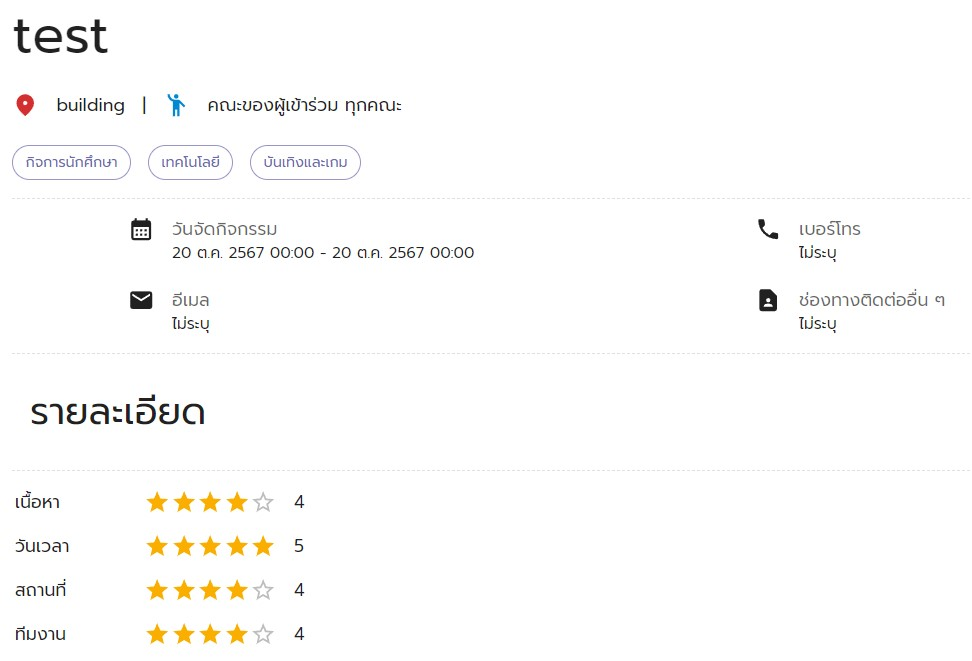
\includegraphics[scale=0.5]{public/act-score.jpg}}
\end{center}
\caption[Poem]{Review Window}
\label{fig:score-section}
\end{figure}


